\documentclass{rvcepaper}
\newcommand{\lgrid}{%
\par\vspace{4pt}\centerline{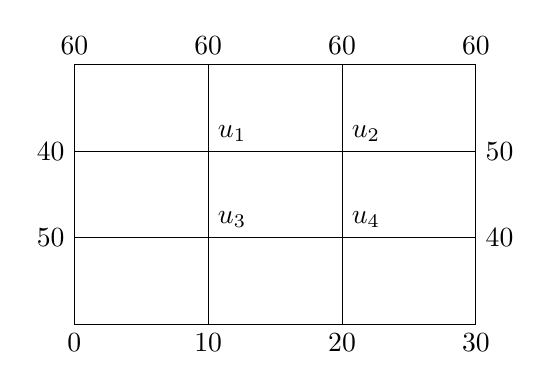
\begin{tikzpicture}[x=1.7cm,y=1.1cm]
 \foreach \i in {0,1,2,3}{\draw (\i,0)--(\i,3); \draw (0,\i)--(3,\i);}
 \foreach \x in {0,1,2,3}{\node[above] at (\x,3) {60};}
 \node[left] at (0,2) {40}; \node[left] at (0,1) {50}; \node[right] at (3,2) {50}; \node[right] at (3,1) {40};
 \node[below] at (0,0) {0}; \node[below] at (1,0) {10}; \node[below] at (2,0) {20}; \node[below] at (3,0) {30};
 \node at (1,2) [above right] {$u_1$}; \node at (2,2) [above right] {$u_2$}; \node at (1,1) [above right] {$u_3$}; \node at (2,1) [above right] {$u_4$};
\end{tikzpicture}}\par\vspace{2pt}}
\begin{document}

%%%%%%%%%%%%%%%%%%%%%%%%%%%% MATHEMATICS
% ---------- MA231TB CIE - III (Improvement Test), 07.01.2025
\begin{xpaper}
\paperinfo{deptline={Department of Mathematics},date={07.01.2025},exam={CIE -- III (Improvement Test)},maxmarks={10 + 50},sem={III},prog={AS, BT, CH, ME, IEM},duration={9.30 AM -- 11.30 AM},
 title={Statistics, Laplace Transform and Numerical Methods},code={MA231TB}}
\xhead
\begin{xtable}{Questions}
\qpart{Part -- A}
\q{1}{The real and imaginary parts of the complex valued function $f(z) = e^z$ is \blank[1.8cm].}{2}{1}{1}
\q{2}{For the 1-D heat equation $\dfrac{\partial u}{\partial t} = 2\dfrac{\partial^2u}{\partial x^2}$ subjected to the boundary conditions $u(0,t) = 0$, $u(4,t) = 0$ for $t > 0$ and initial conditions $u(x,0) = x(4-x)$, $0 < x < 4$, with $\alpha = 1/2$ and h = 1, then the value of $u_{1,2}$ = \blank[1.8cm].}{2}{3}{2}
\q{3}{Find the value of the constants a, b if the function $f(z) = (ax^4 + bx^2y^2 + y^4 + 2x^2 - 2y^2) + i(4x^3y - 4xy^3 + 4xy)$ is analytic.}{2}{2}{2}
\q{4}{For the one-dimensional wave equation $\dfrac{\partial^2u}{\partial t^2} = \dfrac{\partial^2u}{\partial x^2}$, with the boundary conditions $u(0,t) = u(5,t) = 0$, and the initial conditions $u(x,0) = x(x-5)$ and $u_t(x,0) = 0$ with h = 1, k = 1, the value of $u(1,1)$ is \blank[1.8cm].}{2}{3}{2}
\q{5}{The Taylor's series expansion of $f(z) = \cos z$ about z = 0 is \blank[1.8cm].}{2}{2}{1}
\qpart{Part -- B}
\q{1}{Determine the complex potential function $f(z) = u + iv$, given that $2u + v = e^x[\cos(y) - \sin(y)]$. Also find the velocity potential u and stream function v.}{10}{2}{3}
\q{2a}{Verify the function $v = x^2 - y^2 + \dfrac{x}{x^2+y^2}$ is harmonic.}{3}{1}{2}
\q{2b}{Find an analytic function $f(z) = u + iv$ given that $v = \left(r - \dfrac{1}{r}\right)\sin\theta$, $r \ne 0$. Also find u.}{7}{2}{2}
\q{3}{Represent $\dfrac{1}{(z+1)(z+3)}$ as Laurent's series valid in the region (i) $1 < |z| < 3$ (ii) $|z| > 3$ (iii) $0 < |z+1| < 2$ (iv) $|z| < 1$.}{10}{4}{2}
\q{4}{The transverse displacement u of a point at a distance x from one end and at any time t of a vibrating string satisfies the equation $16\dfrac{\partial^2u}{\partial x^2} - \dfrac{\partial^2u}{\partial t^2} = 0$, with boundary conditions $u(0,t) = u(5,t) = 0$ and the initial conditions $u(x,0) = \begin{cases} 3x, & 0 \le x \le \frac{5}{2}\\ 20 - 4x, & \frac{5}{2} \le x \le 5\end{cases}$ and $\dfrac{\partial u}{\partial t} = 0$ at t = 0. Solve the equation numerically up to t = 1, taking h = 1 and k = 1/4.}{10}{3}{3}
\q{5}{Determine the values of $u(x,t)$ satisfying the parabolic equation $\dfrac{\partial u}{\partial t} = 4\dfrac{\partial^2u}{\partial x^2}$ and the boundary conditions $u(0,t) = u(8,t) = 0$ and $u(x,0) = 4x - \dfrac{x^2}{2}$ at the points x = i : i = 0, 1, 2, \ldots, 8 and t = $\dfrac{j}{8}$ : j = 0, 1, 2, \ldots, 5.}{10}{3}{--}
\end{xtable}
\end{xpaper}

% ---------- MA231TB Improvement Test, 19/03/2024
\begin{xpaper}
\paperinfo{deptline={Department of Mathematics},date={19/03/2024},exam={Improvement Test},maxmarks={50},sem={III (AS, BT, CH, IM, ME)},prog={UG},duration={10.00 AM -- 11.30 AM},
 title={Statistics, Laplace Transforms and Numerical Methods},code={MA231TB}}
\xhead
\begin{xtable}{Questions}
\q{1(a)}{Find the Laplace transform of $e^{2t}(3t^5 - \cos 4t)$.}{5}{1}{1}
\q{1(b)}{Find the Laplace transform of $\dfrac{e^{at} - \cos bt}{t}$.}{5}{2}{2}
\q{2(a)}{Express the following function in terms of unit step function and hence find the Laplace transform of $f(t) = \begin{cases} 2t & \text{for } 0 < t < \pi\\ 1 & \text{for } t > \pi\end{cases}$.}{5}{2}{2}
\q{2(b)}{Solve the parabolic equation $\dfrac{\partial^2u}{\partial x^2} = \dfrac{\partial u}{\partial t}$ with the conditions $u(0,t) = u(1,t) = 0$, $u(x,0) = x(1-x)$. Assume $\Delta x = h = 0.2$. Tabulate $u(x,t)$ for 3 levels of time using Bendre Schmidt Method.}{5}{3}{3}
\q{3}{Find the solution of one-dimensional wave equation $u_{tt} = u_{xx}$ up to t = 0.5 with a spacing of $\Delta x = h = 0.1$ and $\Delta t = k = 0.1$ subject to $u(0,t) = 0$, $u(1,t) = 0$, $u_t(x,0) = 0$ and $u(x,0) = 10 + x(1-x)$.}{10}{3}{3}
\q{4}{The temperature distribution $u(x,t)$ is modelled as one-dimensional heat equation $\dfrac{1}{4}u_t = u_{xx}$ for $0 \le x \le 4$ subject to the boundary conditions $u(0,t) = u(4,t) = 0$ and initial condition $u(x,0) = \dfrac{x(4-x)}{2}$. Determine the temperature distribution $u(x,t)$ by taking $\Delta x = h = 1$ and $\Delta t = k = \dfrac{1}{16}$ using Schmidt relation for 4 levels.}{10}{3}{4}
\q{5}{Solve the Laplace equation $u_{xx} + u_{yy} = 0$ given the square mesh (Carry out five iterations).
\lgrid}{10}{3}{3}
\end{xtable}
\end{xpaper}

%%%%%%%%%%%%%%%%%%%%%%%%%%%% WORK SYSTEMS DESIGN
% ---------- IM233AI Improvement Test, January 2025
\begin{iempaper}
\paperinfo{dept={INDUSTRIAL ENGINEERING \& MANAGEMENT},date={January 2025},exam={Improvement Test},maxmarks={50},sem={III},prog={UG},duration={90 Min},
 title={WORK SYSTEMS DESIGN},code={IM233AI}}
\iemhead
\begin{cietable}{M}{BT}{CO}
\qpart{Part -- A}
\q{1}{Sketch a typical physical work system.}{02}{2}{1}
\q{2}{Distinguish between production and productivity.}{02}{2}{1}
\q{3}{Illustrate the pyramidal structure of a task.}{02}{2}{1}
\q{4}{What is meant by the term Poka-Yoke?}{02}{2}{2}
\q{5}{List the five steps in 5S system.}{02}{1}{2}
\qpart{Part -- B}
\q{1}{A work group of 20 workers in a certain month produced 8600 units of output working 8 hr/day for 21 days. (i) What is the labor productivity ratio for this month? (ii) In the next month, the same work group produced 8000 units but there were 22 workdays in the month and the size of the work group was reduced to 14 workers. What is the labor productivity ratio for this second month? (iii) What is the productivity index using the first month as a base?}{10}{4}{1}
\q{2}{The standard time is to be established for a manual work cycle by direct time study. The observed time for the cycle averaged 4.80 minutes. The worker's performance was rated at 90\% on all cycles observed. After eight cycles, the worker must exchange parts containers which took 1.60 minutes rated at 120\%. The PFD allowance for this class of work is 15\%. Determine the normal time, the standard time for the cycle and the worker's efficiency if the worker produces 123 work units during an 8 hour shift.}{10}{4}{1}
\q{3}{In Toyota Production System a standardized work procedure for a given task has three components. What are they? Explain any two in detail.}{10}{2}{2}
\q{4}{Sketch the structure of Lean Production System. Explain the features of different elements of the structure.}{10}{3}{2}
\q{5}{Distinguish between Push System of production control and Pull System of production control. Support your answer with an appropriate illustration.}{10}{3}{2}
\end{cietable}
\end{iempaper}

% ---------- IM233AI Improvement Test, 20th March 2024
\begin{iempaper}
\paperinfo{dept={INDUSTRIAL ENGINEERING \& MANAGEMENT},date={20\textsuperscript{th} March 2024},exam={Improvement Test},maxmarks={50},sem={III},prog={UG},duration={90 Min},
 title={WORK SYSTEMS DESIGN},code={IM233AI}}
\iemhead
\begin{cietable}{M}{BT}{CO}
\q{1}{A work group of 12 workers in a certain month produced 1400 units of output working 8 hr/day for 18 days in the month. What productivity measures could be used for this situation? Suppose that in the next month, the same work group produced 1690 units but there were only 12 work days in the month. Using the same productivity measures as before, determine the productivity index using the prior month as a base.}{10}{3}{1}
\q{2}{A worker performs a repetitive assembly task at a work branch at a work bench to assemble products. Each product consists of 25 components. Various hand tools are used in the task. The standard time for the work cycle is 7.45 minutes, based on using a PFD allowance factor of 15\%. If the worker completes 75 product units during an 8 hour shift, determine the number of standard hours accomplished and the worker efficiency. If the worker took only one rest break, lasting 13 minutes and experienced no other interruptions during the 8 hours of shift time, determine the worker performance.}{10}{4}{3}
\q{3}{Illustrate the structure of Lean Production System. Explain the features of different elements of the structure.}{10}{3}{2}
\q{4}{List all the forms of waste as advocated by Taiichi Ohno in a production environment. Elaborate on any three forms in detail.}{10}{3}{2}
\q{5}{Summarize the prerequisites for a successful implementation of Just in Time philosophy.}{10}{2}{2}
\end{cietable}
\end{iempaper}

% ---------- 21IM33 CIE - Improvement, 21st March 2023
\begin{iempaper}
\paperinfo{dept={INDUSTRIAL ENGINEERING \& MANAGEMENT},date={21\textsuperscript{st} March 2023},exam={CIE -- Improvement},maxmarks={10 + 50},sem={III},prog={UG},duration={20 + 90 Min},
 title={WORK SYSTEMS DESIGN},code={21IM33}}
\iemhead
\begin{cietable}{M}{BT}{CO}
\qpart{Part -- A}
\q{1}{Standard Time is also known as Allowed Time. Justify.}{02}{2}{3}
\q{2}{Distinguish between First generation and Higher generation levels of PMTS.}{02}{2}{3}
\q{3}{List the prerequisites for valid time standards.}{02}{1}{3}
\q{4}{What are the broad two components of Environment in the context and scope of Ergonomics analysis?}{02}{1}{4}
\q{5}{Classify the three basic categories of Human-Machine systems.}{02}{2}{4}
\qpart{Part -- B}
\q{1}{Review different types of Allowances used in Time Standards. Justify the need to consider the same in determining standard times.}{10}{4}{3}
\q{2}{The observed average time in a direct time study was 2.40 minutes for a repetitive work cycle. The worker's performance was rated at 110\% on all cycles. The personal time, fatigue and delay allowance for this work is 12\%. Determine the normal time and the standard time for the cycle.}{10}{3}{3}
\q{3}{The snap back timing method in direct time study was used to obtain the elemental times for a worker machine task as indicated. Element c is a machine controlled and the time is constant. Elements a, b, d, e and f are operator controlled and external to machine cycle and they are performance rated at 80\%. If the machine allowance is 25\% and worker PFD allowance is 15\%, determine the normal time and standard time for the work cycle.
\qtabc{|l|c|c|c|c|c|c|}{\hline Element & a & b & c & d & e & f\\\hline Observed Time (min) & 0.18 & 0.30 & 0.88 & 1.12 & 1.55 & 1.80\\\hline}}{10}{4}{3}
\q{4}{Illustrate and Explain through a block diagram model, the typical interactions in a human-machine system.}{10}{3}{4}
\q{5}{Distinguish between the terms, Hazard and Accident. Also illustrate a model depicting the possible factors that contribute to industrial accidents.}{10}{3}{4}
\end{cietable}
\end{iempaper}

% ---------- 18IM35 CIE - III, November 2019
\begin{xpaper}
\paperinfo{deptline={Department of Industrial Engineering and Management},date={November 2019},exam={CIE -- III},maxmarks={50},sem={III},prog={UG},duration={90 Min},
 title={Work Systems Design},code={18IM35}}
\xhead
\begin{xtable}{Questions (Part -- B)}
\q{1}{Illustrate the role of personal computers and personal digital assistants in computerizing the steps for direct time study.}{10}{3}{4}
\q{2}{Evaluate the role of expert systems in computerized work measurement systems.}{10}{4}{4}
\q{3}{Elaborate the possible contributions to Learning, by the organizations as a part of their continuous improvement strategy.}{10}{2}{1}
\q{4}{Illustrate the structure of a Lean Production System. Elaborate on the features of two pillars in the structure.}{10}{3}{4}
\q{5}{In Toyota Production System a standardized work procedure for a given task has three components. What are they? Explain any two in detail.}{10}{2}{4}
\end{xtable}
\end{xpaper}

%%%%%%%%%%%%%%%%%%%%%%%%%%%% MANUFACTURING PROCESSES
% ---------- IM234AI Improvement CIE, 8th January 2025
\begin{iempaper}
\paperinfo{dept={INDUSTRIAL ENGINEERING \& MANAGEMENT},date={8\textsuperscript{th} January 2025},exam={Improvement CIE},maxmarks={10 + 50},sem={III},prog={UG},duration={120 Min},
 title={MANUFACTURING PROCESSES},code={IM234AI}}
\iemhead
\begin{cietable}{M}{BT}{CO}
\qpart{Part -- A}
\q{1}{For drilling operation, the drill rotates with \blank[1.8cm] pressure if job is held on earth.}{1}{1}{2}
\q{2}{Point angle of drill is also known as \blank[1.8cm].}{1}{1}{3}
\q{3}{In drilling, depth of cut is \blank[1.8cm] the drill diameter.}{1}{2}{2}
\q{4}{Cemented carbides tools are generally manufactured by \blank[1.8cm] technique.}{1}{1}{3}
\q{5}{A tool had life of 10 min with cutting speed 300 m/min. Find the cutting speed for the same tool to have a life of 150 min. Taken $-$0.2 in Taylor's tool life equation.}{2}{2}{2}
\q{6}{State the difference between up and down milling.}{2}{2}{3}
\q{7}{What are the advantages of Twist drill, specify any two.}{2}{1}{3}
\qpart{Part -- B}
\q{1}{List cutting tool materials? Describe in brief, stating its principal characteristics \& application of any four cutting tool materials.}{10}{2}{2}
\q{2}{Sketch and explain the nomenclature of a twist drill.}{10}{2}{3}
\q{3}{Write a short note on the following drilling operations: (i) Reaming (ii) Counter sinking.}{10}{1}{3}
\q{4}{Draw a neat diagram of a Radial Drilling Machine. Name all the parts and explain the principle of operation.}{10}{2}{2}
\q{5}{Explain following milling operation with relevant sketches: (i) Form milling (ii) Gang milling.}{10}{1}{3}
\end{cietable}
\end{iempaper}

% ---------- IM234AI Improvement Test, 20th March 2024
\begin{iempaper}
\paperinfo{dept={INDUSTRIAL ENGINEERING \& MANAGEMENT},date={20\textsuperscript{th} March 2024},exam={Improvement Test},maxmarks={50},sem={III},prog={UG},duration={90 Min},
 title={MANUFACTURING PROCESS},code={IM234AI}}
\iemhead
\begin{cietable}{M}{BT}{CO}
\q{1}{Examine the geometry of a twist drill and its impact on drilling operations.}{10}{1}{1}
\q{2}{List three common types of drills used in a drilling machine. Provide a brief description of each drill type and their typical applications.}{10}{2}{2}
\q{3}{Differentiate between up milling and down milling.}{10}{3}{3}
\q{4}{Show the calculations for setting dividing head to mill 69 divisions on a spur wheel blank by compound indexing?}{10}{2}{2}
\q{5}{Determine time taken for plain milling a rectangular surface of length 100 mm and width 50 mm by a helical fluted plain HSS milling cutter of diameter 60 mm, length 75 mm and 6 teeth. Assume A = O = 5 mm, V$_C$ = 40 m/min and s$_o$ = 0.1 mm/tooth.}{10}{3}{3}
\end{cietable}
\end{iempaper}

% ---------- 21IM34 Improvement Test, 21st March 2023
\begin{iempaper}
\paperinfo{dept={INDUSTRIAL ENGINEERING AND MANAGEMENT},date={21\textsuperscript{st} March 2023},exam={Improvement Test},maxmarks={10 + 50},sem={III},prog={UG},duration={20 + 90 Min},
 title={MANUFACTURING PROCESS},code={21IM34}}
\iemhead
\begin{cietable}{M}{BT}{CO}
\qpart{Part -- A}
\q{1.1}{In chemical machining is material removal happens with the help of \blank[1.8cm].}{01}{2}{3}
\q{1.2}{In the Electro Chemical Machining process, there is the tool and work piece. Which is the Cathode in the configuration?}{01}{1}{4}
\q{1.3}{List any two features of advanced machining process.}{02}{2}{3}
\q{1.4}{In AJM, which of the materials are used as abrasive grains?}{02}{1}{2}
\q{1.5}{Define Hybrid Machining processes.}{02}{2}{3}
\q{1.6}{Summarize difference between EBM and LBM.}{02}{3}{4}
\qpart{Part -- B}
\q{1}{Classify the different types of advanced Machining Processes used in the Industries.}{10}{2}{3}
\q{2}{Draw the schematic diagram and explain the principle of operation of electrochemical grinding process.}{10}{2}{2}
\q{3}{With the aid of sketch, explain the working principle of Water-jet Machining.}{10}{3}{4}
\q{4}{Describe the working principle and construction of laser jet machining.}{10}{2}{3}
\q{5}{State the differences between additive and subtractive manufacturing.}{10}{3}{4}
\end{cietable}
\end{iempaper}

% ---------- 18IM36 CIE - III, November 2019
\begin{xpaper}
\paperinfo{deptline={Department of Industrial Engineering and Management},date={November 2019},exam={CIE -- III},maxmarks={60},sem={III},prog={UG},duration={120 Min},
 title={Manufacturing Process},code={18IM36}}
\xhead
\begin{xtable}{Questions (Part -- B)}
\q{1}{How is skeleton of the bus being manufactured? Explain briefly with the help of the sketch.}{(10)}{4}{2}
\q{2}{What properties determine the quality of a sand mold for sand casting?}{(10)}{2}{2}
\q{3}{Draw the neat sketch of tool layout for producing a bushes in a capstan/turret lathe.}{(10)}{4}{2}
\q{4}{``Moulding processes to produce internal cavities and reentrant angles''. What is the process called and explain the different types.}{(10)}{2}{1}
\q{5}{What are general defects encountered in casting process?}{(10)}{1}{1}
\end{xtable}
\end{xpaper}

%%%%%%%%%%%%%%%%%%%%%%%%%%%% DIGITAL METROLOGY
% ---------- IM235AI Improvement CIE, 9th January 2025
\begin{iempaper}
\paperinfo{dept={INDUSTRIAL ENGINEERING \& MANAGEMENT},date={9\textsuperscript{th} January 2025},exam={Improvement CIE},maxmarks={10 + 50},sem={III},prog={UG},duration={120 Min},
 title={DIGITAL METROLOGY},code={IM235AI}}
\iemhead
\begin{cietable}{M}{BT}{CO}
\qpart{Part -- A}
\q{1}{What are the key components of a CMM system?}{02}{1}{4}
\q{2}{How does a computer-aided inspection system improve the accuracy of measurements in CMMs?}{01}{2}{4}
\q{3}{What is the principle of Interferometry used in optical flats for surface measurement?}{02}{2}{3}
\q{4}{Define the Ten-Point Height Average Value in surface finish analysis.}{01}{1}{3}
\q{5}{How do progressive and periodic errors impact the performance of threaded components, in terms of their functionality and precision?}{02}{2}{3}
\q{6}{How can alignment errors be detected using an autocollimator?}{02}{2}{4}
\qpart{Part -- B}
\q{1}{Describe the principle of interference and its role in precision measurement. Explain the construction and operation of a Tool Maker's Microscope, highlighting its significance in precise dimensional analysis.}{10}{3}{3}
\q{2}{Define Pitch Circle diameter, addendum and dedendum and represent on a gear profile. How can a Vernier Gear Tooth Caliper be used to measure the thickness of a gear tooth? Explain the procedure briefly.}{10}{3}{3}
\q{3}{Discuss the Tomlinson Surface Meter, its construction, principles of operation, and applications in surface finish measurement. Explain how this specialized instrument contributes to accurate surface finish analysis in engineering and manufacturing processes, highlighting its advantages and limitations.}{10}{3}{3}
\q{4}{Describe the Michelson Interferometer and its working principles in detail, highlighting its key components and the interference phenomena it utilizes. Discuss the applications of Michelson Interferometers in various fields.}{10}{3}{4}
\q{5}{Discuss the different types of CMMs and their applications in industrial inspection.}{10}{2}{4}
\end{cietable}
\end{iempaper}

% ---------- 22IM325AI Improvement Test, 22nd March 2024
\begin{iempaper}
\paperinfo{dept={INDUSTRIAL ENGINEERING \& MANAGEMENT},date={22\textsuperscript{nd} March 2024},exam={Improvement Test},maxmarks={50},sem={III},prog={UG},duration={90 Min},
 title={DIGITAL METROLOGY},code={22IM325AI}}
\iemhead
\begin{cietable}{M}{BT}{CO}
\q{1}{Explain the functioning of a tactile sensors and Piezoelectric sensor, detailing its basic operation and how it detects contact with surfaces. Provide examples of applications where these sensors are commonly used.}{10}{3}{2}
\q{2}{Discuss six key specifications of sensors and describe briefly the operational principles of Potentiometer Sensors. Provide a detailed explanation of how Potentiometer Sensors function and illustrate their applications.}{10}{3}{2}
\q{3}{Explain briefly the 4 main elements of a Coordinate Measuring Machine (CMM).}{10}{2}{4}
\q{4}{How does Coordinate Measuring Machine (CMM) integration with Computer-Aided Manufacturing (CAM) enhance quality control processes in manufacturing? Discuss with examples.}{10}{3}{4}
\q{5}{Describe the Michelson Interferometer and its working principles in detail, highlighting its key components and the interference phenomena it utilizes. Discuss the applications of Michelson Interferometers in various fields.}{10}{2}{4}
\end{cietable}
\end{iempaper}

% ---------- 18IM34 CIE - III, November 2019
\begin{xpaper}
\paperinfo{deptline={Department of Industrial Engineering and Management},date={November 2019},exam={CIE -- III},maxmarks={50},sem={III},prog={UG},duration={90 Min},
 title={Metrology and Measurements},code={18IM34}}
\xhead
\begin{xtable}{Questions}
\q{Q1}{Explain briefly the Operating principle of a Autocollimator and describe how it can be used for the measurement of straightness.}{(10)}{--}{--}
\q{Q2}{Explain briefly the working principle of a sine bar and with neat sketches, describe the uses of it.}{(10)}{--}{--}
\q{Q3a}{With neat sketches explain briefly any three systems of displacement amplification used in Mechanical Comparators.}{(06)}{--}{--}
\q{Q3b}{Explain the basic principle of a Pneumatic comparator.}{(04)}{--}{--}
\q{Q4}{``LVDT works on the principle of Mutual Induction'' -- Explain briefly its working with neat sketches and list any four applications of it.}{(10)}{--}{--}
\q{Q5}{Explain the basic principle of LASER. List the various uses of LASER in metrology and explain any two in detail.}{10}{--}{--}
\end{xtable}
\end{xpaper}

%%%%%%%%%%%%%%%%%%%%%%%%%%%% BASKET / OTHER-DEPARTMENT COURSES
% ---------- ME232TB Material Science for Engineers, CIE - Improvement Test, January 2025
\begin{xpaper}
\paperinfo{deptline={Department of Mechanical Engineering},date={January 2025},exam={CIE -- Improvement Test},maxmarks={50 + 10},sem={III},prog={UG},duration={120 Min},
 title={Material Science for Engineers},code={ME232TB}}
\xhead
\begin{xtable}{Questions}
\qpart{Part A (Quiz)}
\q{1}{Mention the main purpose of annealing heat treatment process of ferrous materials.}{1}{1}{3}
\q{2}{In \blank[1.8cm] type of annealing, the lamellar pearlite is transformed into globular type structure.}{1}{1}{3}
\q{3}{In pack (solid) carburizing \blank[1.8cm] is used as energizer.}{1}{1}{3}
\q{4}{Give two examples for 1D nanomaterial.}{2}{1}{3}
\q{5}{What happens to the elastic modulus property, when the material brought to nanoscale?}{1}{1}{4}
\q{6}{Name two top-down methods of nano-material synthesis.}{2}{2}{4}
\q{7}{In sol-gel process the formation of an oxide network takes place through \blank[1.8cm] reactions of a molecular precursor in the liquid.}{1}{1}{4}
\q{8}{Mesoporous materials are a class of nanomaterials characterized by their highly ordered porous structure with pore sizes ranging from \blank[1.5cm] to \blank[1.5cm] nanometers.}{1}{1}{4}
\qpart{Part B (Test)}
\q{1a)}{Describe the normalizing heat treatment process with the help of a neat sketch.}{05}{2}{3}
\q{1b)}{Discuss the flame hardening process with a neat sketch.}{05}{2}{3}
\q{2}{Illustrate the construction of TTT diagram for eutectoid steel of 0.8\% carbon with neat sketches and label various features on the diagram. Also state the applications of the TTT diagram.}{10}{3}{3}
\q{3a)}{Enumerate the purposes of post-processing heat treatment methods of electronic devices.}{05}{3}{3}
\q{3b)}{Explain the rapid thermal processing with a neat sketch with its advantages.}{05}{3}{3}
\q{4}{``Identify whether the chemical vapour deposition (CVD) is top-down or bottom-up approach''. Justify your answer and explain the working principle with the help of neat sketch. State its applications and advantages.}{10}{3}{4}
\q{5}{Discuss the working principle and various modes of atomic force microscope (AFM) with neat sketches.}{10}{3}{4}
\end{xtable}
\end{xpaper}

% ---------- ME232AT Materials Science for Engineers, CIE - Improvement, March 2024
\begin{xpaper}
\paperinfo{deptline={Department of Mechanical Engineering},date={March 2024},exam={CIE -- Improvement},maxmarks={50},sem={3},prog={UG},duration={90 Min},
 title={Materials Science for Engineers},code={ME232AT}}
\xhead
\begin{xtable}{Questions}
\q{1a.}{Define heat treatment and explain the purpose of heat treatment.}{5}{2}{3}
\q{1b.}{Discuss the advantages and applications of rapid thermal processing for electronic devices.}{5}{2}{3}
\q{2a.}{Differentiate between annealing and normalising heat treatment processes.}{5}{3}{3}
\q{2b.}{Describe the full annealing heat treatment process for ferrous materials.}{5}{3}{3}
\q{3a.}{Explain the steps involved in thermal oxidation of semiconductor devices.}{6}{3}{3}
\q{3b.}{Describe the defects of heat treatment process for different materials.}{4}{2}{3}
\q{4.}{With the help of TTT diagram explain hardening process.}{10}{3}{3}
\q{5.}{Explain the following heat treatment processes with neat sketches: i) Flame hardening and ii) carburising.}{10}{3}{3}
\end{xtable}
\end{xpaper}

% ---------- CV232AT Environment and Sustainability, CIE - III (Test), 19-03-2024
\begin{xpaper}
\paperinfo{deptline={Department of Civil Engineering},date={19-03-2024},exam={CIE -- III (Test)},maxmarks={50},sem={III},prog={UG},duration={90 Min},
 title={Environment and Sustainability},code={CV232AT}}
\xhead
\begin{xtable}{Questions}
\q{1a}{Enumerate the impacts of ozone layer depletion.}{5}{2}{3}
\q{1b}{Explain the concept of 5R.}{5}{2}{3}
\q{2}{Define the following. i) EIA ii) Climate change iii) Carbon Credit iv) Carbon Footprint v) Green Building.}{10}{2}{3}
\q{3}{Explain the principles of CSR.}{10}{2}{4}
\q{4}{Enumerate the ways to reduce carbon foot print.}{10}{3}{3}
\q{5a}{Briefly explain the concept of circular economy.}{5}{2}{3}
\q{5b}{Explain the concept of charity and corporate philanthropy.}{5}{2}{4}
\end{xtable}
\end{xpaper}

% ---------- BT232AT Bio Safety Standards and Ethics, Improvement Test, 8th January 2025
\begin{xpaper}
\paperinfo{deptline={Department of Biotechnology},date={8\textsuperscript{th} January 2025},exam={Improvement Test},maxmarks={60},sem={III},prog={UG},duration={120 Min},
 title={Bio Safety Standards and Ethics (Basket Course)},code={BT232AT}}
\xhead
\begin{xtable}{Questions (Quiz)}
\q{1}{What is food processing?}{1}{1}{3}
\q{2}{What is Innovative Packaging? Give examples.}{1}{1}{3}
\q{3}{What are the advantages of preservation of food?}{1}{1}{3}
\q{4}{What are flavouring agents used in food? Give examples.}{1}{1}{4}
\q{5}{List out the health policies in India.}{1}{1}{4}
\q{6}{What is food safety?}{1}{1}{4}
\q{7}{What is ethics in food industry?}{2}{1}{4}
\q{8}{List out 4 methods used for food analysis.}{2}{1}{4}
\end{xtable}
\par\vspace{4pt}
\begin{xtable}{Questions (Test)}
\q{1}{Classify food preservatives, explain the strategies used for various foods preservation.}{10}{2}{3}
\q{2}{Illustrate and classify on various food packaging methods used in food industry.}{10}{3}{4}
\q{3}{``Meat and meat products derived from livestock treated with antibiotics and hormones can cause adverse effects on consumer's health'' justify the statement.}{10}{3}{3}
\q{4}{Elaborate on smart packaging methods with suitable examples. Add a note on packaging materials.}{10}{4}{4}
\q{5}{Write explanatory notes on: Clinical Ethics and Research Ethics.}{5 + 5}{2}{3}
\end{xtable}
\end{xpaper}

% ---------- BT232AT Bio Safety Standards and Ethics, Closed Book Offline Test - 3 (2023-24)
\begin{xpaper}
\paperinfo{deptline={Department of Biotechnology},date={2023-24 (Odd Sem)},exam={Closed Book Offline Test -- 3},maxmarks={50},sem={III},prog={UG},duration={--},
 title={Bio Safety Standards and Ethics (Basket Course)},code={BT232AT}}
\xhead
\begin{xtable}{Questions (Test)}
\q{1}{Explain on various food processing techniques.}{10}{2}{4}
\q{2}{Illustrate on the following: Blanching, Pasteurization, Frying.}{10}{4}{4}
\q{3}{Describe three levels of packaging the food products.}{10}{4}{4}
\q{4}{Explain the effects of poor packaging on food products, add a note on smart packing.}{10}{2}{4}
\q{5}{Write Explanatory notes on: Freezing, Dehydration, Homogenization.}{10}{2}{4}
\end{xtable}
\end{xpaper}

\end{document}
